\documentclass[]{tufte-handout}

% ams
\usepackage{amssymb,amsmath}

\usepackage{ifxetex,ifluatex}
\usepackage{fixltx2e} % provides \textsubscript
\ifnum 0\ifxetex 1\fi\ifluatex 1\fi=0 % if pdftex
  \usepackage[T1]{fontenc}
  \usepackage[utf8]{inputenc}
\else % if luatex or xelatex
  \makeatletter
  \@ifpackageloaded{fontspec}{}{\usepackage{fontspec}}
  \makeatother
  \defaultfontfeatures{Ligatures=TeX,Scale=MatchLowercase}
  \makeatletter
  \@ifpackageloaded{soul}{
     \renewcommand\allcapsspacing[1]{{\addfontfeature{LetterSpace=15}#1}}
     \renewcommand\smallcapsspacing[1]{{\addfontfeature{LetterSpace=10}#1}}
   }{}
  \makeatother

\fi

% graphix
\usepackage{graphicx}
\setkeys{Gin}{width=\linewidth,totalheight=\textheight,keepaspectratio}

% booktabs
\usepackage{booktabs}

% url
\usepackage{url}

% hyperref
\usepackage{hyperref}

% units.
\usepackage{units}


\setcounter{secnumdepth}{-1}

% citations
\usepackage{natbib}
\bibliographystyle{plainnat}

% pandoc syntax highlighting
\usepackage{color}
\usepackage{fancyvrb}
\newcommand{\VerbBar}{|}
\newcommand{\VERB}{\Verb[commandchars=\\\{\}]}
\DefineVerbatimEnvironment{Highlighting}{Verbatim}{commandchars=\\\{\}}
% Add ',fontsize=\small' for more characters per line
\newenvironment{Shaded}{}{}
\newcommand{\AlertTok}[1]{\textcolor[rgb]{1.00,0.00,0.00}{\textbf{#1}}}
\newcommand{\AnnotationTok}[1]{\textcolor[rgb]{0.38,0.63,0.69}{\textbf{\textit{#1}}}}
\newcommand{\AttributeTok}[1]{\textcolor[rgb]{0.49,0.56,0.16}{#1}}
\newcommand{\BaseNTok}[1]{\textcolor[rgb]{0.25,0.63,0.44}{#1}}
\newcommand{\BuiltInTok}[1]{#1}
\newcommand{\CharTok}[1]{\textcolor[rgb]{0.25,0.44,0.63}{#1}}
\newcommand{\CommentTok}[1]{\textcolor[rgb]{0.38,0.63,0.69}{\textit{#1}}}
\newcommand{\CommentVarTok}[1]{\textcolor[rgb]{0.38,0.63,0.69}{\textbf{\textit{#1}}}}
\newcommand{\ConstantTok}[1]{\textcolor[rgb]{0.53,0.00,0.00}{#1}}
\newcommand{\ControlFlowTok}[1]{\textcolor[rgb]{0.00,0.44,0.13}{\textbf{#1}}}
\newcommand{\DataTypeTok}[1]{\textcolor[rgb]{0.56,0.13,0.00}{#1}}
\newcommand{\DecValTok}[1]{\textcolor[rgb]{0.25,0.63,0.44}{#1}}
\newcommand{\DocumentationTok}[1]{\textcolor[rgb]{0.73,0.13,0.13}{\textit{#1}}}
\newcommand{\ErrorTok}[1]{\textcolor[rgb]{1.00,0.00,0.00}{\textbf{#1}}}
\newcommand{\ExtensionTok}[1]{#1}
\newcommand{\FloatTok}[1]{\textcolor[rgb]{0.25,0.63,0.44}{#1}}
\newcommand{\FunctionTok}[1]{\textcolor[rgb]{0.02,0.16,0.49}{#1}}
\newcommand{\ImportTok}[1]{#1}
\newcommand{\InformationTok}[1]{\textcolor[rgb]{0.38,0.63,0.69}{\textbf{\textit{#1}}}}
\newcommand{\KeywordTok}[1]{\textcolor[rgb]{0.00,0.44,0.13}{\textbf{#1}}}
\newcommand{\NormalTok}[1]{#1}
\newcommand{\OperatorTok}[1]{\textcolor[rgb]{0.40,0.40,0.40}{#1}}
\newcommand{\OtherTok}[1]{\textcolor[rgb]{0.00,0.44,0.13}{#1}}
\newcommand{\PreprocessorTok}[1]{\textcolor[rgb]{0.74,0.48,0.00}{#1}}
\newcommand{\RegionMarkerTok}[1]{#1}
\newcommand{\SpecialCharTok}[1]{\textcolor[rgb]{0.25,0.44,0.63}{#1}}
\newcommand{\SpecialStringTok}[1]{\textcolor[rgb]{0.73,0.40,0.53}{#1}}
\newcommand{\StringTok}[1]{\textcolor[rgb]{0.25,0.44,0.63}{#1}}
\newcommand{\VariableTok}[1]{\textcolor[rgb]{0.10,0.09,0.49}{#1}}
\newcommand{\VerbatimStringTok}[1]{\textcolor[rgb]{0.25,0.44,0.63}{#1}}
\newcommand{\WarningTok}[1]{\textcolor[rgb]{0.38,0.63,0.69}{\textbf{\textit{#1}}}}

% longtable

% multiplecol
\usepackage{multicol}

% strikeout
\usepackage[normalem]{ulem}

% morefloats
\usepackage{morefloats}


% tightlist macro required by pandoc >= 1.14
\providecommand{\tightlist}{%
  \setlength{\itemsep}{0pt}\setlength{\parskip}{0pt}}

% title / author / date
\title{Marketing Report}
\date{2020-03-19}

\usepackage{booktabs}
\usepackage{longtable}
\usepackage{array}
\usepackage{multirow}
\usepackage{wrapfig}
\usepackage{float}
\usepackage{colortbl}
\usepackage{pdflscape}
\usepackage{tabu}
\usepackage{threeparttable}
\usepackage{threeparttablex}
\usepackage[normalem]{ulem}
\usepackage{makecell}
\usepackage{xcolor}

\begin{document}

\maketitle




\hypertarget{description}{%
\section{Description}\label{description}}

In anticipation of an evaluation of third party inquiry vendors, I was
asked to provide a summary of Cappex and Hobson's performance over the
past three years.

Cappex and Hobson contract details are as follows:

\begin{itemize}
\item
  Cappex - annual contract, November - October, 16,500 USD
\item
  Hobson - 29,643.02 USD

  \begin{itemize}
  \item
    Intersect Awareness: annual contract, for the enhanced college
    profile and counselor community: October - September
  \item
    Intersect Connection-Active match competitive: 6 mos: August -
    January
  \item
    Intersect Connection-Active match self matching: 6 mos: August -
    January
  \end{itemize}
\end{itemize}

\hypertarget{findings}{%
\section{Findings}\label{findings}}

\begin{table}

\caption{\label{tab:unnamed-chunk-3} Total Inquiries by Contract Period}
\centering
\begin{tabu} to \linewidth {>{\raggedright}X>{\raggedleft}X>{\raggedleft}X>{\raggedleft}X>{\raggedleft}X>{\raggedleft}X}
\toprule
Initial.Referral.Source & Inquired & Applied & Admitted & Confirmed & Enrolled\\
\midrule
\addlinespace[0.3em]
\multicolumn{6}{l}{\textbf{Contract 2016 - 2017}}\\
\hspace{1em}CPPX & 1181 & 207 & 189 & 69 & 60\\
\hspace{1em}HBSN & 715 & 210 & 174 & 51 & 41\\
\addlinespace[0.3em]
\multicolumn{6}{l}{\textbf{Contract 2017 - 2018}}\\
\hspace{1em}CPPX & 971 & 138 & 118 & 35 & 27\\
\hspace{1em}HBSN & 628 & 329 & 282 & 89 & 72\\
\addlinespace[0.3em]
\multicolumn{6}{l}{\textbf{Contract 2018 - 2019}}\\
\hspace{1em}CPPX & 1326 & 223 & 214 & 19 & 4\\
\hspace{1em}HBSN & 407 & 135 & 116 & 28 & 15\\
\addlinespace[0.3em]
\multicolumn{6}{l}{\textbf{Contract 2019 - 2020}}\\
\hspace{1em}CPPX & 229 & 19 & 17 & 0 & 0\\
\hspace{1em}HBSN & 535 & 171 & 150 & 5 & 0\\
\bottomrule
\end{tabu}
\end{table}

\begin{table}

\caption{\label{tab:unnamed-chunk-4}Total Inquiries by Anticipated Start Year}
\centering
\begin{tabu} to \linewidth {>{\raggedright}X>{\raggedleft}X>{\raggedleft}X>{\raggedleft}X>{\raggedleft}X>{\raggedleft}X}
\toprule
Initial.Referral.Source & Inquired & Applied & Admitted & Confirmed & Enrolled\\
\midrule
\addlinespace[0.3em]
\multicolumn{6}{l}{\textbf{Anticipated Start 2017}}\\
\hspace{1em}CPPX & 230 & 17 & 14 & 7 & 6\\
\hspace{1em}HBSN & 403 & 69 & 52 & 8 & 7\\
\addlinespace[0.3em]
\multicolumn{6}{l}{\textbf{Anticipated Start 2018}}\\
\hspace{1em}CPPX & 807 & 118 & 111 & 41 & 36\\
\hspace{1em}HBSN & 515 & 238 & 205 & 61 & 52\\
\addlinespace[0.3em]
\multicolumn{6}{l}{\textbf{Anticipated Start  2019}}\\
\hspace{1em}CPPX & 824 & 114 & 101 & 34 & 29\\
\hspace{1em}HBSN & 672 & 297 & 252 & 85 & 68\\
\addlinespace[0.3em]
\multicolumn{6}{l}{\textbf{Anticipated Start 2020}}\\
\hspace{1em}CPPX & 1386 & 337 & 311 & 41 & 20\\
\hspace{1em}HBSN & 596 & 241 & 213 & 19 & 1\\
\addlinespace[0.3em]
\multicolumn{6}{l}{\textbf{Anticipated Start 2021}}\\
\hspace{1em}CPPX & 367 & 1 & 1 & 0 & 0\\
\hspace{1em}HBSN & 95 & 0 & 0 & 0 & 0\\
\addlinespace[0.3em]
\multicolumn{6}{l}{\textbf{Anticipated Start 2022}}\\
\hspace{1em}CPPX & 84 & 0 & 0 & 0 & 0\\
\hspace{1em}HBSN & 4 & 0 & 0 & 0 & 0\\
\bottomrule
\end{tabu}
\end{table}

\begin{table}

\caption{\label{tab:unnamed-chunk-5}Cappex Inquiries by Contract Period}
\centering
\begin{tabu} to \linewidth {>{\raggedright}X>{\raggedright}X>{\raggedleft}X>{\raggedleft}X>{\raggedleft}X>{\raggedleft}X>{\raggedleft}X}
\toprule
  & Anticipated.Start & Inquired & Applied & Admitted & Confirmed & Enrolled\\
\midrule
\addlinespace[0.3em]
\multicolumn{7}{l}{\textbf{Contract CPPX 2016 - 2017}}\\
\hspace{1em}1 & Fall 2017 & 225 & 17 & 14 & 7 & 6\\
\hspace{1em}2 & Fall 2018 & 576 & 106 & 101 & 37 & 34\\
\hspace{1em}3 & Fall 2019 & 326 & 52 & 46 & 16 & 13\\
\hspace{1em}4 & Fall 2020 & 51 & 31 & 27 & 9 & 7\\
\hspace{1em}5 & Fall 2021 & 3 & 1 & 1 & 0 & 0\\
\addlinespace[0.3em]
\multicolumn{7}{l}{\textbf{Contract CPPX 2017 - 2018}}\\
\hspace{1em}6 & Fall 2017 & 2 & 0 & 0 & 0 & 0\\
\hspace{1em}7 & Fall 2018 & 223 & 12 & 10 & 4 & 2\\
\hspace{1em}8 & Fall 2019 & 410 & 57 & 50 & 16 & 15\\
\hspace{1em}9 & Fall 2020 & 314 & 69 & 58 & 15 & 10\\
\hspace{1em}10 & Fall 2021 & 22 & 0 & 0 & 0 & 0\\
\addlinespace[0.3em]
\multicolumn{7}{l}{\textbf{Contract CPPX 2018 - 2019}}\\
\hspace{1em}13 & Fall 2019 & 88 & 5 & 5 & 2 & 1\\
\hspace{1em}14 & Fall 2020 & 916 & 218 & 209 & 17 & 3\\
\hspace{1em}15 & Fall 2021 & 256 & 0 & 0 & 0 & 0\\
\hspace{1em}16 & Fall 2022 & 46 & 0 & 0 & 0 & 0\\
\addlinespace[0.3em]
\multicolumn{7}{l}{\textbf{Contract CPPX 2019 - 2020}}\\
\hspace{1em}18 & Fall 2020 & 105 & 19 & 17 & 0 & 0\\
\hspace{1em}19 & Fall 2021 & 86 & 0 & 0 & 0 & 0\\
\hspace{1em}20 & Fall 2022 & 38 & 0 & 0 & 0 & 0\\
\bottomrule
\end{tabu}
\end{table}

\begin{table}

\caption{\label{tab:unnamed-chunk-6}Hobson Inquiries by Contract Period}
\centering
\begin{tabu} to \linewidth {>{\raggedright}X>{\raggedright}X>{\raggedleft}X>{\raggedleft}X>{\raggedleft}X>{\raggedleft}X>{\raggedleft}X}
\toprule
  & Anticipated.Start & Inquired & Applied & Admitted & Confirmed & Enrolled\\
\midrule
\addlinespace[0.3em]
\multicolumn{7}{l}{\textbf{Contract HBSN 2016 - 2017}}\\
\hspace{1em}1 & Fall 2017 & 403 & 69 & 52 & 8 & 7\\
\hspace{1em}2 & Fall 2018 & 287 & 126 & 112 & 38 & 31\\
\hspace{1em}3 & Fall 2019 & 19 & 11 & 9 & 5 & 3\\
\hspace{1em}4 & Fall 2020 & 6 & 4 & 1 & 0 & 0\\
\addlinespace[0.3em]
\multicolumn{7}{l}{\textbf{Contract HBSN 2017 - 2018}}\\
\hspace{1em}5 & Fall 2018 & 228 & 112 & 93 & 23 & 21\\
\hspace{1em}6 & Fall 2019 & 381 & 202 & 177 & 59 & 50\\
\hspace{1em}7 & Fall 2020 & 18 & 15 & 12 & 7 & 1\\
\addlinespace[0.3em]
\multicolumn{7}{l}{\textbf{Contract HBSN 2018 - 2019}}\\
\hspace{1em}9 & Fall 2019 & 272 & 84 & 66 & 21 & 15\\
\hspace{1em}10 & Fall 2020 & 129 & 51 & 50 & 7 & 0\\
\hspace{1em}11 & Fall 2021 & 6 & 0 & 0 & 0 & 0\\
\addlinespace[0.3em]
\multicolumn{7}{l}{\textbf{Contract HBSN 2019 - 2020}}\\
\hspace{1em}12 & Fall 2020 & 443 & 171 & 150 & 5 & 0\\
\hspace{1em}13 & Fall 2021 & 88 & 0 & 0 & 0 & 0\\
\hspace{1em}14 & Fall 2022 & 4 & 0 & 0 & 0 & 0\\
\bottomrule
\end{tabu}
\end{table}

\begin{table}

\caption{\label{tab:unnamed-chunk-8} Total Inquiries and Enrollments by State 2016-2020}
\centering
\begin{tabu} to \linewidth {>{\raggedright}X>{\raggedright}X>{\raggedleft}X>{\raggedleft}X}
\toprule
Region & Initial.Referral.Source & Inquired & Enrolled\\
\midrule
\addlinespace[0.3em]
\multicolumn{4}{l}{\textbf{Maine}}\\
\hspace{1em}Maine & CPPX & 981 & 71\\
\hspace{1em}Maine & HBSN & 744 & 111\\
\addlinespace[0.3em]
\multicolumn{4}{l}{\textbf{New Hampshire}}\\
\hspace{1em}New Hampshire & CPPX & 290 & 8\\
\hspace{1em}New Hampshire & HBSN & 215 & 2\\
\addlinespace[0.3em]
\multicolumn{4}{l}{\textbf{Massachusetts}}\\
\hspace{1em}Massachusetts & CPPX & 500 & 3\\
\hspace{1em}Massachusetts & HBSN & 601 & 4\\
\addlinespace[0.3em]
\multicolumn{4}{l}{\textbf{Connecticut}}\\
\hspace{1em}Connecticut & CPPX & 314 & 2\\
\hspace{1em}Connecticut & HBSN & 194 & 4\\
\addlinespace[0.3em]
\multicolumn{4}{l}{\textbf{Vermont}}\\
\hspace{1em}Vermont & CPPX & 82 & 4\\
\hspace{1em}Vermont & HBSN & 98 & 4\\
\addlinespace[0.3em]
\multicolumn{4}{l}{\textbf{Rhode Island}}\\
\hspace{1em}Rhode Island & CPPX & 96 & 0\\
\hspace{1em}Rhode Island & HBSN & 1 & 0\\
\addlinespace[0.3em]
\multicolumn{4}{l}{\textbf{Other}}\\
\hspace{1em}Other & CPPX & 1446 & 3\\
\hspace{1em}Other & HBSN & 432 & 3\\
\bottomrule
\end{tabu}
\end{table}

\hypertarget{anticipated-start-2017}{%
\subsubsection{Anticipated Start 2017}\label{anticipated-start-2017}}

\begin{table}

\caption{\label{tab:unnamed-chunk-9}Fall 2017: Total Inquiries and Enrollments by State}
\centering
\begin{tabu} to \linewidth {>{\raggedright}X>{\raggedright}X>{\raggedleft}X>{\raggedleft}X}
\toprule
Region & Initial.Referral.Source & Inquired & Enrolled\\
\midrule
\addlinespace[0.3em]
\multicolumn{4}{l}{\textbf{Maine}}\\
\hspace{1em}Maine & CPPX & 26 & 2\\
\hspace{1em}Maine & HBSN & 21 & 5\\
\addlinespace[0.3em]
\multicolumn{4}{l}{\textbf{New Hampshire}}\\
\hspace{1em}New Hampshire & CPPX & 7 & 1\\
\hspace{1em}New Hampshire & HBSN & 17 & 0\\
\addlinespace[0.3em]
\multicolumn{4}{l}{\textbf{Massachusetts}}\\
\hspace{1em}Massachusetts & CPPX & 26 & 2\\
\hspace{1em}Massachusetts & HBSN & 111 & 0\\
\addlinespace[0.3em]
\multicolumn{4}{l}{\textbf{Connecticut}}\\
\hspace{1em}Connecticut & CPPX & 11 & 0\\
\hspace{1em}Connecticut & HBSN & 23 & 1\\
\addlinespace[0.3em]
\multicolumn{4}{l}{\textbf{Vermont}}\\
\hspace{1em}Vermont & CPPX & 7 & 1\\
\hspace{1em}Vermont & HBSN & 9 & 1\\
\addlinespace[0.3em]
\multicolumn{4}{l}{\textbf{Rhode Island}}\\
\hspace{1em}Rhode Island & CPPX & 3 & 0\\
\addlinespace[0.3em]
\multicolumn{4}{l}{\textbf{Other}}\\
\hspace{1em}Other & CPPX & 150 & 0\\
\hspace{1em}Other & HBSN & 222 & 0\\
\bottomrule
\end{tabu}
\end{table}

\hypertarget{anticipated-start-2018}{%
\subsubsection{Anticipated Start 2018}\label{anticipated-start-2018}}

\begin{table}

\caption{\label{tab:unnamed-chunk-10}Fall 2018: Total Inquiries and Enrollments by State}
\centering
\begin{tabu} to \linewidth {>{\raggedright}X>{\raggedright}X>{\raggedleft}X>{\raggedleft}X}
\toprule
Region & Initial.Referral.Source & Inquired & Enrolled\\
\midrule
\addlinespace[0.3em]
\multicolumn{4}{l}{\textbf{Maine}}\\
\hspace{1em}Maine & CPPX & 198 & 28\\
\hspace{1em}Maine & HBSN & 224 & 47\\
\addlinespace[0.3em]
\multicolumn{4}{l}{\textbf{New Hampshire}}\\
\hspace{1em}New Hampshire & CPPX & 86 & 4\\
\hspace{1em}New Hampshire & HBSN & 58 & 0\\
\addlinespace[0.3em]
\multicolumn{4}{l}{\textbf{Massachusetts}}\\
\hspace{1em}Massachusetts & CPPX & 134 & 0\\
\hspace{1em}Massachusetts & HBSN & 134 & 1\\
\addlinespace[0.3em]
\multicolumn{4}{l}{\textbf{Connecticut}}\\
\hspace{1em}Connecticut & CPPX & 78 & 1\\
\hspace{1em}Connecticut & HBSN & 35 & 0\\
\addlinespace[0.3em]
\multicolumn{4}{l}{\textbf{Vermont}}\\
\hspace{1em}Vermont & CPPX & 23 & 3\\
\hspace{1em}Vermont & HBSN & 22 & 1\\
\addlinespace[0.3em]
\multicolumn{4}{l}{\textbf{Rhode Island}}\\
\hspace{1em}Rhode Island & CPPX & 22 & 0\\
\hspace{1em}Rhode Island & HBSN & 1 & 0\\
\addlinespace[0.3em]
\multicolumn{4}{l}{\textbf{Other}}\\
\hspace{1em}Other & CPPX & 266 & 0\\
\hspace{1em}Other & HBSN & 41 & 3\\
\bottomrule
\end{tabu}
\end{table}

\hypertarget{anticipated-start-2019}{%
\subsubsection{Anticipated Start 2019}\label{anticipated-start-2019}}

\begin{table}

\caption{\label{tab:unnamed-chunk-11}Fall 2019: Total Inquiries and Enrollments by State}
\centering
\begin{tabu} to \linewidth {>{\raggedright}X>{\raggedright}X>{\raggedleft}X>{\raggedleft}X}
\toprule
Region & Initial.Referral.Source & Inquired & Enrolled\\
\midrule
\addlinespace[0.3em]
\multicolumn{4}{l}{\textbf{Maine}}\\
\hspace{1em}Maine & CPPX & 200 & 25\\
\hspace{1em}Maine & HBSN & 265 & 58\\
\addlinespace[0.3em]
\multicolumn{4}{l}{\textbf{New Hampshire}}\\
\hspace{1em}New Hampshire & CPPX & 71 & 3\\
\hspace{1em}New Hampshire & HBSN & 72 & 2\\
\addlinespace[0.3em]
\multicolumn{4}{l}{\textbf{Massachusetts}}\\
\hspace{1em}Massachusetts & CPPX & 135 & 0\\
\hspace{1em}Massachusetts & HBSN & 180 & 3\\
\addlinespace[0.3em]
\multicolumn{4}{l}{\textbf{Connecticut}}\\
\hspace{1em}Connecticut & CPPX & 104 & 0\\
\hspace{1em}Connecticut & HBSN & 73 & 3\\
\addlinespace[0.3em]
\multicolumn{4}{l}{\textbf{Vermont}}\\
\hspace{1em}Vermont & CPPX & 21 & 0\\
\hspace{1em}Vermont & HBSN & 27 & 2\\
\addlinespace[0.3em]
\multicolumn{4}{l}{\textbf{Rhode Island}}\\
\hspace{1em}Rhode Island & CPPX & 28 & 0\\
\addlinespace[0.3em]
\multicolumn{4}{l}{\textbf{Other}}\\
\hspace{1em}Other & CPPX & 265 & 1\\
\hspace{1em}Other & HBSN & 55 & 0\\
\bottomrule
\end{tabu}
\end{table}

\hypertarget{anticipated-start-2020}{%
\subsubsection{Anticipated Start 2020}\label{anticipated-start-2020}}

\begin{table}

\caption{\label{tab:unnamed-chunk-12}Fall 2020: Total Inquiries and Enrollments by State}
\centering
\begin{tabu} to \linewidth {>{\raggedright}X>{\raggedright}X>{\raggedleft}X>{\raggedleft}X>{\raggedleft}X>{\raggedleft}X}
\toprule
Region & Initial.Referral.Source & Inquired & Applied & Admitted & Enrolled\\
\midrule
\addlinespace[0.3em]
\multicolumn{6}{l}{\textbf{Maine}}\\
\hspace{1em}Maine & CPPX & 464 & 234 & 215 & 16\\
\hspace{1em}Maine & HBSN & 222 & 149 & 135 & 1\\
\addlinespace[0.3em]
\multicolumn{6}{l}{\textbf{New Hampshire}}\\
\hspace{1em}New Hampshire & CPPX & 89 & 20 & 19 & 0\\
\hspace{1em}New Hampshire & HBSN & 53 & 18 & 17 & 0\\
\addlinespace[0.3em]
\multicolumn{6}{l}{\textbf{Massachusetts}}\\
\hspace{1em}Massachusetts & CPPX & 149 & 28 & 26 & 1\\
\hspace{1em}Massachusetts & HBSN & 144 & 33 & 26 & 0\\
\addlinespace[0.3em]
\multicolumn{6}{l}{\textbf{Connecticut}}\\
\hspace{1em}Connecticut & CPPX & 88 & 9 & 9 & 1\\
\hspace{1em}Connecticut & HBSN & 51 & 21 & 18 & 0\\
\addlinespace[0.3em]
\multicolumn{6}{l}{\textbf{Vermont}}\\
\hspace{1em}Vermont & CPPX & 21 & 6 & 6 & 0\\
\hspace{1em}Vermont & HBSN & 36 & 13 & 12 & 0\\
\addlinespace[0.3em]
\multicolumn{6}{l}{\textbf{Rhode Island}}\\
\hspace{1em}Rhode Island & CPPX & 32 & 7 & 7 & 0\\
\addlinespace[0.3em]
\multicolumn{6}{l}{\textbf{Other}}\\
\hspace{1em}Other & CPPX & 543 & 33 & 29 & 2\\
\hspace{1em}Other & HBSN & 90 & 7 & 5 & 0\\
\bottomrule
\end{tabu}
\end{table}

\begin{figure*}
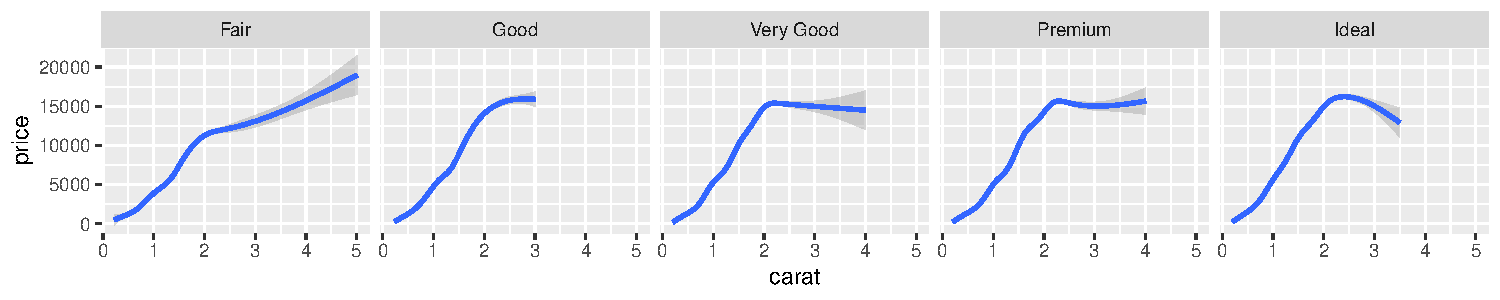
\includegraphics{CPPXHBSN-Comparison_files/figure-latex/fig-fullwidth-1} \caption[This is a full width plot]{This is a full width plot.}\label{fig:fig-fullwidth}
\end{figure*}

\hypertarget{margin-figures}{%
\subsection{Margin Figures}\label{margin-figures}}

Images and graphics play an integral role in Tufte's work. To place
figures in the margin you can use the \textbf{knitr} chunk option
\texttt{fig.margin\ =\ TRUE}. For example:

\begin{marginfigure}
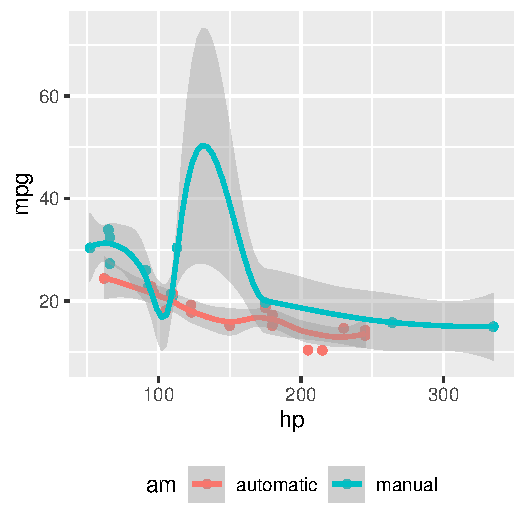
\includegraphics{CPPXHBSN-Comparison_files/figure-latex/fig-margin-1} \caption[MPG vs horsepower, colored by transmission]{MPG vs horsepower, colored by transmission.}\label{fig:fig-margin}
\end{marginfigure}

\hypertarget{sidenotes}{%
\subsection{Sidenotes}\label{sidenotes}}

If you'd like to place ancillary information in the margin without the
sidenote mark (the superscript number), you can use the
\texttt{margin\_note()} function from \textbf{tufte} in an inline R
expression.
\marginnote{This is a margin note.  Notice that there is no number preceding the note.}
This function does not process the text with Pandoc, so Markdown syntax
will not work here. If you need to write anything in Markdown syntax,
please use the \texttt{marginfigure} block described previously.

\hypertarget{tables}{%
\subsection{Tables}\label{tables}}

You can use the \texttt{kable()} function from the \textbf{knitr}
package to format tables that integrate well with the rest of the Tufte
handout style. The table captions are placed in the margin like figures
in the HTML output.

Intro text here Intro text here Intro text here Intro text here Intro
text here Intro text here Intro text here Intro text here. Intro text
here Intro text here Intro text here Intro text here Intro text here
Intro text here Intro text here Intro text here. Intro text here Intro
text here Intro text here Intro text here Intro text here Intro text
here Intro text here Intro text here.

\begin{table}

\caption{\label{tab:unnamed-chunk-13}A subset of mtcars.}
\centering
\begin{tabular}[t]{l|r|r|r|r|r|r}
\hline
  & mpg & cyl & disp & hp & drat & wt\\
\hline
Mazda RX4 & 21.0 & 6 & 160 & 110 & 3.90 & 2.620\\
\hline
Mazda RX4 Wag & 21.0 & 6 & 160 & 110 & 3.90 & 2.875\\
\hline
Datsun 710 & 22.8 & 4 & 108 & 93 & 3.85 & 2.320\\
\hline
Hornet 4 Drive & 21.4 & 6 & 258 & 110 & 3.08 & 3.215\\
\hline
Hornet Sportabout & 18.7 & 8 & 360 & 175 & 3.15 & 3.440\\
\hline
Valiant & 18.1 & 6 & 225 & 105 & 2.76 & 3.460\\
\hline
\end{tabular}
\end{table}

\begin{marginfigure}
Notice that there is no number preceding the note. \(x \in [a, b]\)有
\[\frac{d}{dx}\left( \int_{a}^{x} f(u)\,du\right)=f(x).\]
\end{marginfigure}

\hypertarget{plots-with-margin-notes}{%
\subsection{Plots with Margin Notes}\label{plots-with-margin-notes}}

Intro text here Intro text here Intro text here Intro text here Intro
text here Intro text here Intro text here Intro text here. If you'd like
to place ancillary information in the margin without the sidenote mark
(the superscript number), you can use the \texttt{margin\_note()}
function from \textbf{tufte} in an inline R expression.

\begin{Shaded}
\begin{Highlighting}[]
\KeywordTok{ggplot}\NormalTok{(diamonds, }\KeywordTok{aes}\NormalTok{(cut, price)) }\OperatorTok{+}\StringTok{ }\KeywordTok{geom_boxplot}\NormalTok{()}
\end{Highlighting}
\end{Shaded}

\textbackslash begin\{figure\}
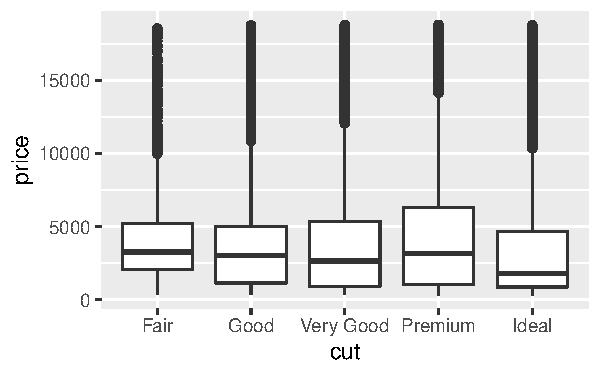
\includegraphics{CPPXHBSN-Comparison_files/figure-latex/fig-main-1}
\textbackslash caption{[}Some general comments about this plot{]}\{Some
general comments about this plot. \$500 Notice the dollar sign
renders.\}\label{fig:fig-main} \textbackslash end\{figure\}

\begin{marginfigure}
Notice that there is no number preceding the note. \(x \in [a, b]\)有
\[\frac{d}{dx}\left( \int_{a}^{x} f(u)\,du\right)=f(x).\]
\end{marginfigure}

\hypertarget{roi}{%
\section{ROI}\label{roi}}

Profit Profit Profit Profit Profit Profit Profit Profit Profit

\hypertarget{conclusion}{%
\section{Conclusion}\label{conclusion}}

\begin{itemize}
\tightlist
\item
  代码段选项
\item
  代码段选项
\item
  代码段选项
\end{itemize}

\bibliography{skeleton.bib}



\end{document}
